% =============================================================================
% Presentación para reunión con Gonzalo — resultados v2 (post-arbitraje
% simulado) y cierre pre-envío a RBEF.
% Compilar (desde docs/): pdflatex presentacion_gonzalo.tex  (dos pasadas)
% Videos que acompañan: videos_reunion/video_N79_v1.16_solido_canales.mp4
%                       videos_reunion/video_N79_v2.0_fusion_canales.mp4
% (dos paneles sincronizados: KE por átomo | ΔPE relativa al equilibrio;
%  fondo claro, Viridis / azul-blanco-rojo. Reemplazan la versión de panel
%  único con fondo negro y paleta Hot.)
% =============================================================================
\documentclass[11pt,aspectratio=169]{beamer}

\usetheme{Madrid}
\usecolortheme{seahorse}
\setbeamertemplate{navigation symbols}{}
\setbeamertemplate{footline}[frame number]

\usepackage[utf8]{inputenc}
\usepackage[T1]{fontenc}
\usepackage[spanish,es-nodecimaldot]{babel}
\usepackage{amsmath,amssymb}
\usepackage{graphicx}
\usepackage{booktabs}

\newcommand{\eps}{\varepsilon}
\newcommand{\lammps}{\textsc{Lammps}}
\newcommand{\pmm}[2]{$#1\!\pm\!#2$}

\title[Rebote de nanocúmulos LJ]{¿A dónde se va la energía de una pelota
que rebota?\\ \large Partición energética del impacto de nanocúmulos LJ
--- resultados finales y cierre pre-envío}
\author[F. Wasaff]{Felipe Wasaff\\
\footnotesize reunión con Gonzalo Gutiérrez}
\institute[IMA-PUCV]{Instituto de Matemáticas, PUCV}
\date{Julio 2026}

\begin{document}

% -----------------------------------------------------------------------------
\begin{frame}
\titlepage
\end{frame}

% -----------------------------------------------------------------------------
\begin{frame}{De dónde venimos y qué hicimos}
\begin{columns}[T]
\column{0.55\textwidth}
\textbf{Punto de partida (2012):} el rebote del cúmulo de
$N\approx79$ átomos de Ar (capítulo \emph{Inelastic Collisions\ldots}).
Aquel análisis describe el balance \emph{durante} el contacto.

\bigskip
\textbf{Lo que hicimos ahora:}
\begin{itemize}
    \item Partición \textbf{al primer apogeo} en 4 canales, cierre exacto
    \item Barrido $N\in\{1,2,7,13,55,79,87\}$ $\times$ 6 alturas
    $\times$ \textbf{5 orientaciones} = 210 corridas, todo con media$\,\pm\,\sigma$
    \item $N_c$ \textbf{medido} en el dump (no ajustado a mano)
    \item Estado de la bola ($T_{\rm ef}$, $g(r)$), test de losa doble,
    simulación larga, caso con adhesión
\end{itemize}
\column{0.42\textwidth}
\begin{block}{La pregunta del paper}
El coeficiente de restitución $e<1$ dice \emph{cuánta} energía no vuelve.
\medskip

¿\textbf{Dónde} queda esa energía justo después del rebote?
¿En la pelota o en el piso?
\end{block}
\begin{alertblock}{Respuesta corta}
En la pelota. Y la fracción sigue una equipartición
--- aplicada a la cantidad correcta.
\end{alertblock}
\end{columns}
\end{frame}

% -----------------------------------------------------------------------------
\begin{frame}{El experimento en una imagen \hfill
\footnotesize[Video 1: \texttt{video\_N79\_v1.16\_solido\_canales.mp4}]}
\begin{center}
    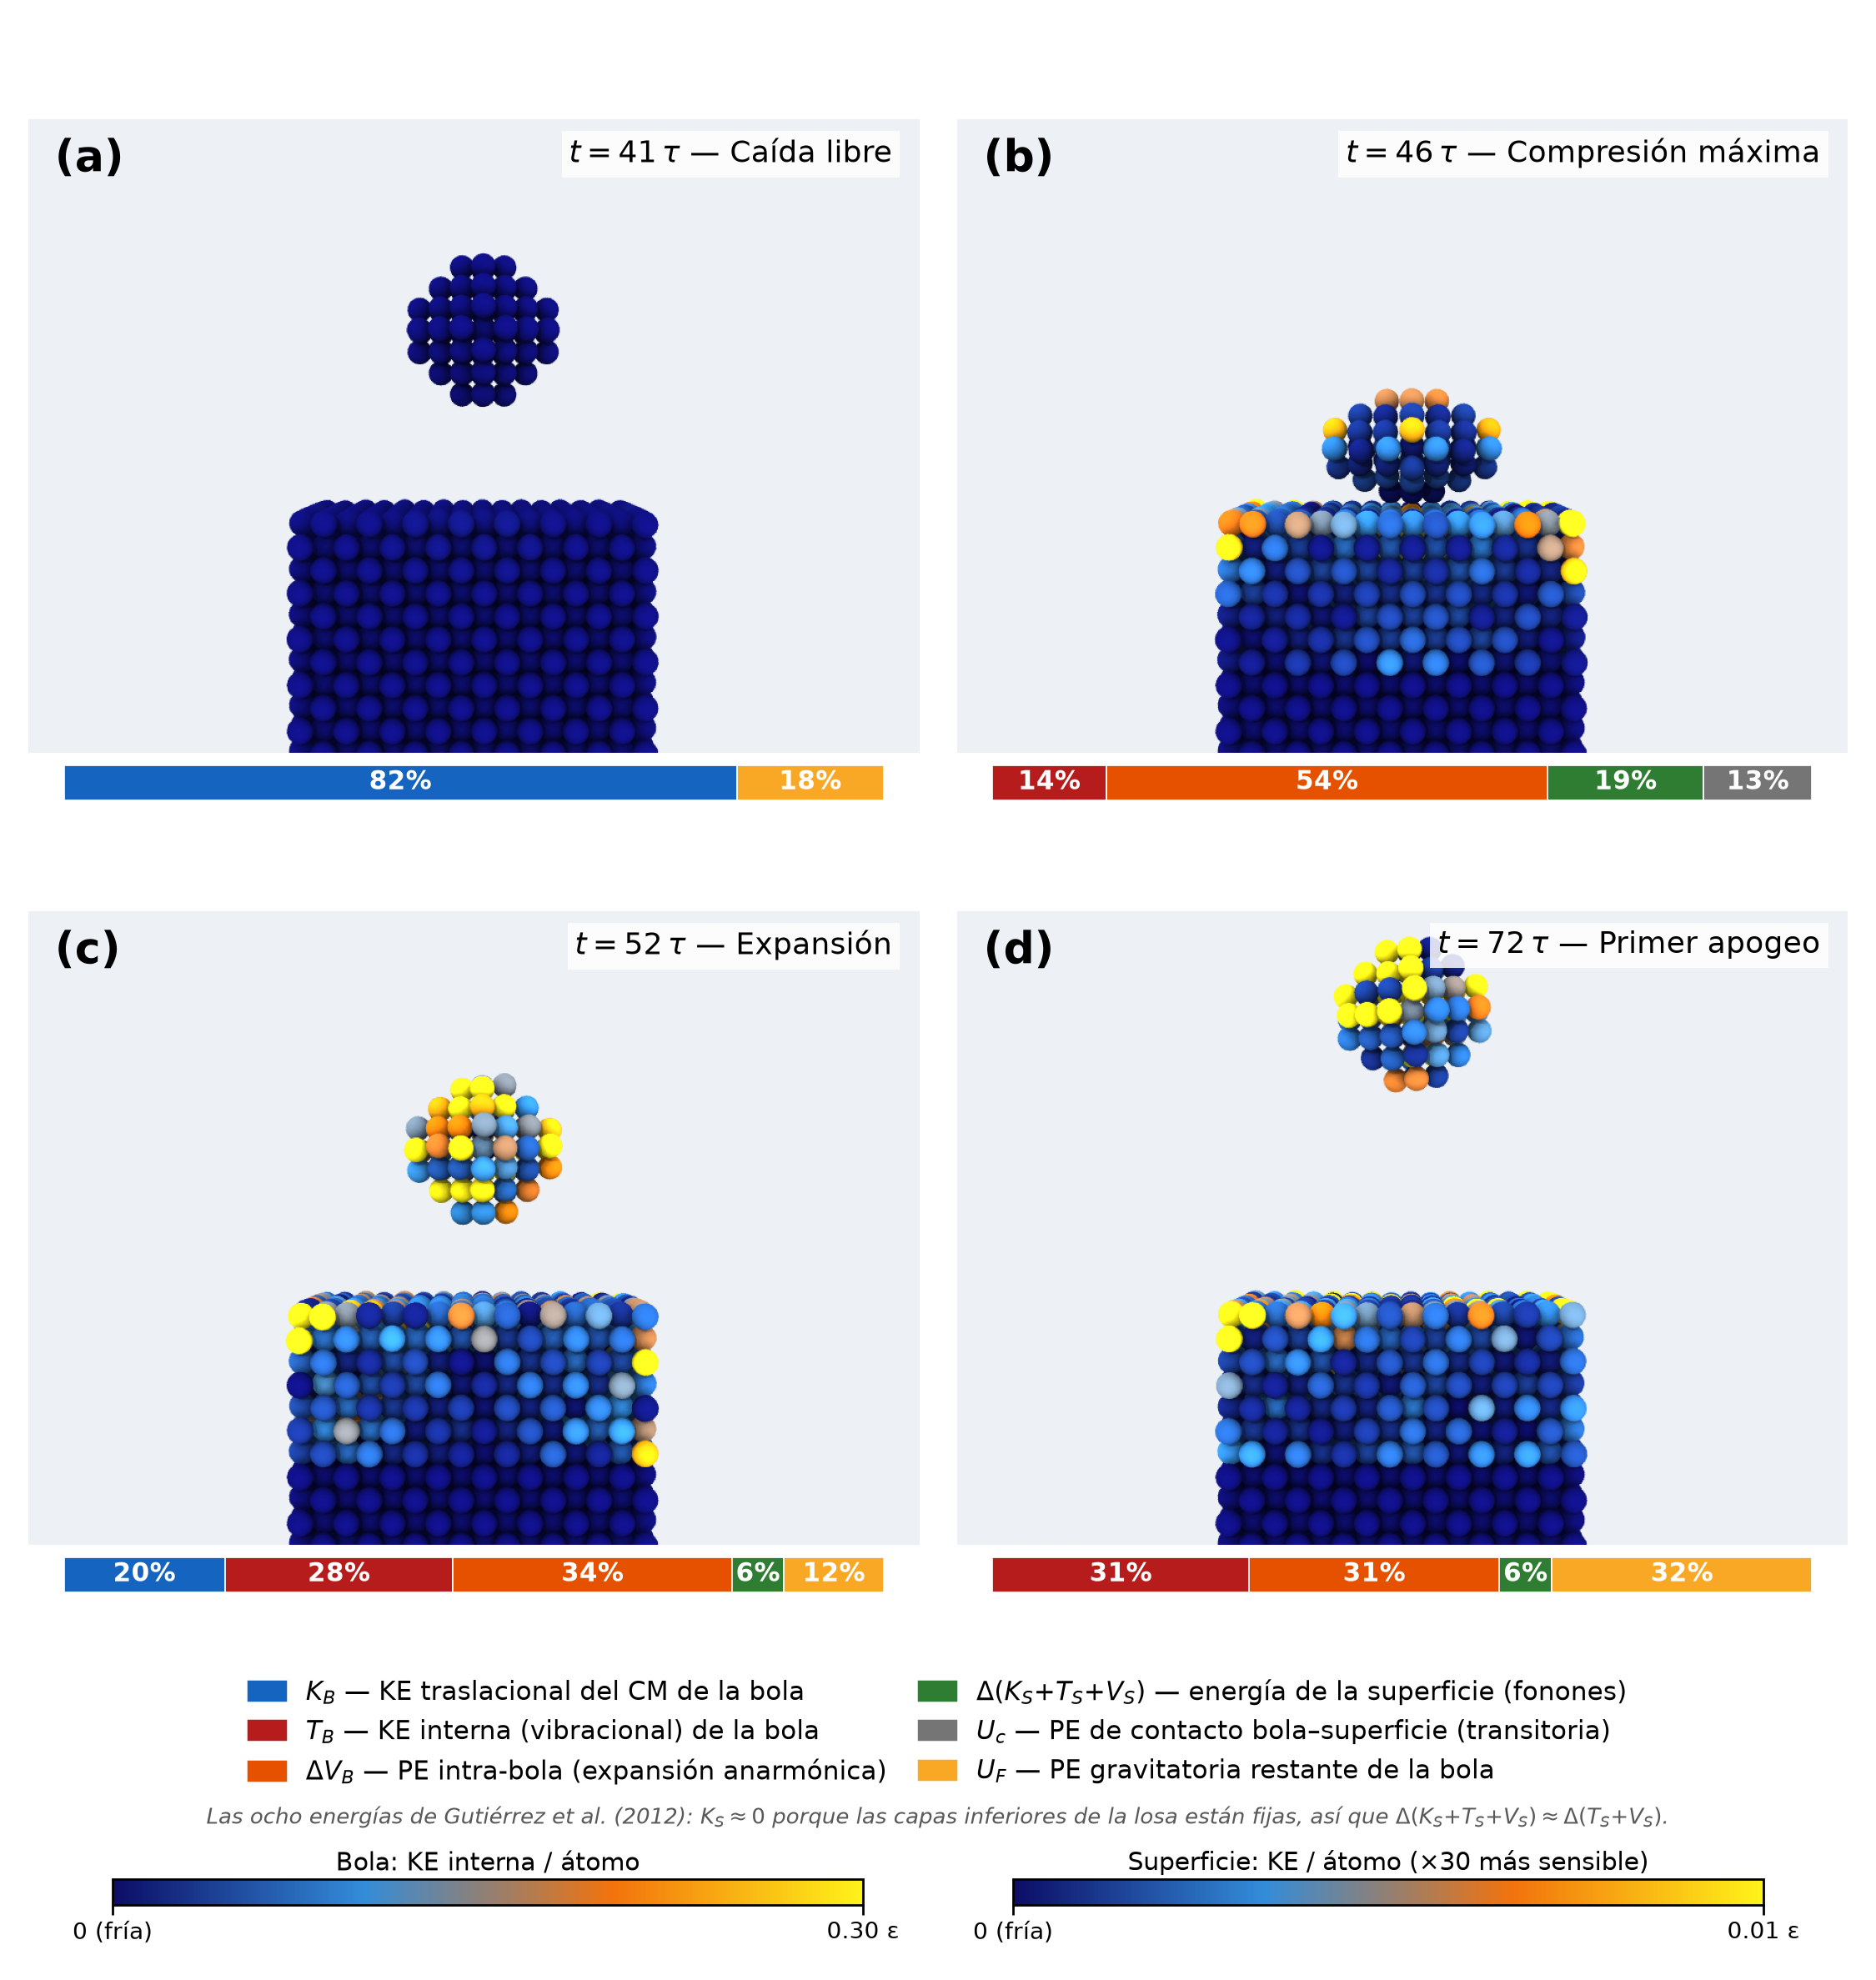
\includegraphics[height=0.8\textheight]{../figuras_rbef/fig_sequence.png}
\end{center}
\end{frame}

% -----------------------------------------------------------------------------
\begin{frame}{Los cuatro canales ($N=79$, repulsivo, $T=0$; 5 orientaciones)}
\begin{columns}[T]
\column{0.60\textwidth}
\scriptsize
\setlength{\tabcolsep}{3.5pt}
\begin{tabular}{cccccc}
\toprule
$v_{\rm imp}$ & $e_1$ & $\alpha_{\rm cm}$ & $\alpha_{T_B}$ &
$\alpha_{\Delta V_B}$ & $\alpha_{\rm surf}$ \\
\midrule
0.70 & \pmm{0.87}{0.05} & \pmm{0.76}{0.08} & \pmm{0.13}{0.09} & \pmm{0.04}{0.02} & \pmm{0.08}{0.02} \\
0.93 & \pmm{0.70}{0.14} & \pmm{0.51}{0.17} & \pmm{0.17}{0.05} & \pmm{0.21}{0.17} & \pmm{0.11}{0.05} \\
1.16 & \pmm{0.62}{0.10} & \pmm{0.40}{0.12} & \pmm{0.22}{0.10} & \pmm{0.24}{0.10} & \pmm{0.14}{0.07} \\
1.43 & \pmm{0.59}{0.06} & \pmm{0.35}{0.06} & \pmm{0.21}{0.06} & \pmm{0.26}{0.09} & \pmm{0.18}{0.09} \\
1.72 & \pmm{0.53}{0.05} & \pmm{0.28}{0.05} & \pmm{0.19}{0.04} & \pmm{0.31}{0.05} & \pmm{0.23}{0.10} \\
2.02 & \pmm{0.49}{0.05} & \pmm{0.24}{0.05} & \pmm{0.18}{0.02} & \pmm{0.31}{0.05} & \pmm{0.27}{0.10} \\
\bottomrule
\end{tabular}

\medskip
\footnotesize $\alpha_{\Delta V_B}$ por cierre; verificado contra $V_B$
directo: solo falta la KE \emph{lateral} del CM
(mediana $5\times10^{-4}E_0$; $<0.02\,E_0$ para $N\ge55$).
\column{0.38\textwidth}
\begin{itemize}
    \item Plateau $\alpha_{T_B}\approx0.22$ para
    $0.9<v\lesssim1.7\,\sigma/\tau$
    \item Canal potencial $\Delta V_B\approx T_B$ (virial: sólido casi
    armónico); el exceso $\Delta V_B-T_B$, creciente con $v$, es la
    parte anarmónica
    \item La superficie se lleva 8--27\%
\end{itemize}
\begin{alertblock}{\small Mensaje central}
\small La energía ``perdida'' queda mayoritariamente
\textbf{dentro de la bola} ($\alpha_{\rm bola}\approx0.4$--$0.6$).
\end{alertblock}
\end{columns}
\end{frame}

% -----------------------------------------------------------------------------
\begin{frame}{Control de calidad I: conservación y dinámica de los canales}
\begin{center}
    \includegraphics[width=0.82\textwidth]{figuras_reunion/fig_conservacion.pdf}
\end{center}
\small (a)~$E_{\rm tot}+U_{\rm grav}$ conservada a
$|\Delta E|=0.023\,\eps=4.3\times10^{-4}E_0$ en $400\,\tau$
($\Delta t=5\times10^{-3}\,\tau$, NVE).
(b)~Canales alrededor del primer impacto ($N=79$, $v=1.16$): $U_c$ es
transitorio; $T_B$ y $\Delta V_B$ quedan en la bola, $\approx$ iguales.
Sin \texttt{pair\_modify shift yes} el cierre fallaba 2--6\% de $E_0$.
\end{frame}

% -----------------------------------------------------------------------------
\begin{frame}{Control de calidad II: termalización de la bola}
\begin{center}
    \includegraphics[width=0.84\textwidth]{figuras_reunion/fig_termalizacion.pdf}
\end{center}
\small (a)~$T_{\rm ef}(t)$: salto en el impacto y equilibrio interno rápido
($\sim10\,\tau$ de contacto $\gg$ período vibracional) --- condición para
hablar de equipartición.
(b)~$T_{\rm ef}$ en el apogeo vs $v_{\rm imp}$: la bola queda \emph{fría}
respecto de la fusión hasta $v\approx1.7$.
\end{frame}

% -----------------------------------------------------------------------------
\begin{frame}{Control de calidad III: validación contra 2012 (Fig.~7 digitalizada)}
\begin{columns}[T]
\column{0.52\textwidth}
\small
\begin{tabular}{c|ccc|cc}
\toprule
 & \multicolumn{3}{c|}{2012 (Fig.~7)} & \multicolumn{2}{c}{2026} \\
$h_0$ & $h_0^{\rm ef}$ & $h_1^{\rm ef}$ & $e_1$ & $h_0^{\rm ef}$ & $e_1$ \\
\midrule
11.03 &  0.6 &  0.4 & ---  &  8.8 & 0.92 \\
18.64 &  8.4 &  6.8 & 0.90 & 17.2 & 0.71 \\
28.15 & 17.9 &  3.3 & 0.43 & 25.9 & 0.55 \\
41.47 & 31.3 &  8.2 & 0.51 & 41.8 & 0.63 \\
58.60 & 48.4 & 14.3 & 0.54 & 56.9 & 0.61 \\
79.53 & 69.2 & 18.2 & 0.51 & 79.0 & 0.59 \\
\bottomrule
\end{tabular}
\column{0.46\textwidth}
\begin{itemize}
    \item \textbf{Hallazgo de convención:} en 2012, $h_0$ = altura
    \emph{absoluta} del CM ($z_{\rm rest}\approx10.3\,\sigma$);
    ahora se mide desde el tope de la losa
    \item A caída efectiva comparable: \textbf{0.90 vs 0.92} en el
    régimen cuasi-elástico
    \item A alta energía, diferencias $\sim0.06$--$0.09$ (cúmulo sin
    minimizar, $N$ variable 79--84, Beeman) --- dentro de la dispersión
    entre orientaciones ($\pm0.05$--$0.14$)
\end{itemize}
\end{columns}
\end{frame}

% -----------------------------------------------------------------------------
\begin{frame}{El argumento que corregimos (y por qué)}
\begin{columns}[T]
\column{0.48\textwidth}
\begin{block}{Versión anterior (inconsistente)}
Equipartición sobre $E_0$ con $N_c=N$:
\[ \alpha_{\rm bola}=\frac{3N-3}{3N-3+3N_c}\;\to\;\tfrac12 \]
Problemas: ignora que el CM no participa del reparto; $N_c$ tenía
\textbf{tres calibraciones} distintas; predice
$\alpha_{\rm surf}\to\tfrac12$, que los datos no muestran.
\end{block}
\column{0.48\textwidth}
\begin{alertblock}{Versión corregida (v2)}
La única energía que se reparte es la \textbf{disipada}, $1-\alpha_{\rm cm}$:
\[ f_{\rm ball}\equiv\frac{\alpha_{\rm bola}}{\alpha_{\rm bola}+\alpha_{\rm surf}}
   =\frac{3N-3}{3N-3+3N_c^{\rm ef}} \]
Con $N_c^{\rm ef}=25\pm8$ \textbf{constante}:
\[ f_{\rm ball}\xrightarrow{N\to\infty}1 \quad(\text{no }1/2). \]
\end{alertblock}
\end{columns}
\medskip
\centering\small El arbitraje interno detectó la inconsistencia; la
medición directa de $N_c$ la resolvió. El resultado corregido es más
limpio \emph{y} más interesante.
\end{frame}

% -----------------------------------------------------------------------------
\begin{frame}{El resultado central: $f_{\rm ball}(N)$ y $N_c^{\rm ef}\approx25$}
\begin{columns}[T]
\column{0.40\textwidth}
\small
\begin{tabular}{cc}
\toprule
$N$ & $f_{\rm ball}$ (plateau) \\
\midrule
2  & \pmm{0.34}{0.29} \\
7  & \pmm{0.55}{0.23} \\
13$^a$ & \pmm{0.38}{0.13} \\
55 & \pmm{0.49}{0.18} \\
79 & \pmm{0.70}{0.14} \\
87 & \pmm{0.77}{0.09} \\
\bottomrule
\end{tabular}

\medskip
\footnotesize $^a$ $N=13$ (y $N=7$): régimen molecular, no termalizan
--- la excepción que confirma el mecanismo.
\column{0.56\textwidth}
\begin{itemize}
    \item Ajuste global con \textbf{una sola constante}:
    $N_c^{\rm ef}=25\pm8$ (honesto: es \emph{ajustado}, pero acotado por
    dos mediciones directas $\to$ próxima lámina)
    \item Una bola grande, fría y sin adhesión retiene \emph{casi toda}
    la energía que no devuelve al CM: sus $3N-3$ modos superan de largo
    la capacidad neta fija de la superficie
    \item Acuerdo cuantitativo para $N\ge55$; cualitativo por debajo
\end{itemize}
\end{columns}
\end{frame}

% -----------------------------------------------------------------------------
\begin{frame}{Por qué $N_c^{\rm ef}$ es tan chico: las tres escalas de $N_c$}
\begin{columns}[T]
\column{0.62\textwidth}
\begin{center}
    \includegraphics[width=\textwidth]{../figuras_rbef/fig_Nc_escalas.pdf}
\end{center}
\column{0.36\textwidth}
\small Medido en el dump ($v\approx1.47$):
\medskip

\footnotesize
\begin{tabular}{@{}ll@{}}
$N_c^{\rm ef}\approx25$ & neto (ajuste) \\[2pt]
\ \ $\ll N_c^{\rm geom}\approx45$--$90$ & huella \\[2pt]
\ \ $\ll N_c^{\rm part}\approx300$--$410$ & particip.\ KE \\
\end{tabular}
\medskip
\begin{itemize}
    \item Cientos de átomos se mueven \emph{transitoriamente}, pero la
    superficie es \textbf{casi elástica}: devuelve la energía al despegue
    \item El viejo $N_c\approx290$ coincidía por accidente con
    $N_c^{\rm part}$: número correcto, balance equivocado
\end{itemize}
\end{columns}
\end{frame}

% -----------------------------------------------------------------------------
\begin{frame}{Límites declarados I: ¿sigue sólida la bola?
\hfill\footnotesize[Video 2: \texttt{video\_N79\_v2.0\_fusion\_canales.mp4}]}
\begin{columns}[T]
\column{0.62\textwidth}
\begin{center}
    \includegraphics[width=\textwidth]{../figuras_rbef/fig_fusion_gr.pdf}
\end{center}
\column{0.36\textwidth}
\small
\begin{itemize}
    \item $v=1.47$: picos FCC nítidos (contraste $\approx11$) --- sólida
    \item $v=2.03$: $g(r)$ colapsada (contraste $\approx2$) --- fundida,
    consistente con la fusión reportada en 2012
    \item Criterio decisivo: $g(r)$ (a $v=2.03$, $T_{\rm ef}=0.28$ queda
    apenas bajo $T^*_{\rm fus}\approx0.30$--$0.35$)
    \item Por eso el plateau y el conteo de modos se restringen a
    $v\lesssim1.7$
\end{itemize}
\end{columns}
\end{frame}

% -----------------------------------------------------------------------------
\begin{frame}{Límites declarados II: tamaño finito de la losa}
\begin{columns}[T]
\column{0.5\textwidth}
\small Test $N=79$, $v\approx1.43$:
\begin{tabular}{lccc}
\toprule
Losa & $\alpha_{\rm surf}$ & $\alpha_{\rm bola}$ & $f_{\rm ball}$ \\
\midrule
$8\times8\times6$    & 0.083 & 0.553 & 0.87 \\
$16\times16\times12$ & 0.143 & 0.435 & 0.75 \\
\bottomrule
\end{tabular}
\column{0.48\textwidth}
\small
\begin{itemize}
    \item El árbitro (simulado) tenía razón: la losa chica
    \textbf{subestima} $\alpha_{\rm surf}$ en $\sim0.06\,E_0$
    (fonones reflejados en fondo fijo y bordes periódicos)
    \item Conclusión robusta: $f_{\rm ball}=0.75$ aun con losa doble
    \item Declarado como sesgo sistemático junto a los datos; un segundo
    caso de control son $\sim$30 min de cómputo si lo pides
\end{itemize}
\end{columns}
\end{frame}

% -----------------------------------------------------------------------------
\begin{frame}{$h^*=T_B/(Mg)$: útil para el primer rebote, no es atractor}
\begin{columns}[T]
\column{0.55\textwidth}
\begin{center}
    \includegraphics[height=0.78\textheight]{../figuras_rbef/fig_paso_B_convergencia.pdf}
\end{center}
\column{0.42\textwidth}
\begin{itemize}
    \item Primer rebote: $h_1/h^* = 0.96$ \checkmark
    \item Rebotes sucesivos: la razón cae monótonamente
    \item Atrapamiento tras 23 rebotes ($t\approx660\,\tau$)
    \item El ``colapso'' posterior a través de la red es un artefacto del
    potencial repulsivo puro (sin barrera lateral), documentado como
    ejercicio de análisis crítico
\end{itemize}
\end{columns}
\end{frame}

% -----------------------------------------------------------------------------
\begin{frame}{Con adhesión ($c_{ps}=1$): la bola siempre pega}
\begin{columns}[T]
\column{0.55\textwidth}
\begin{center}
    \includegraphics[width=\textwidth]{../figuras_rbef/fig_paso_C_adhesion.pdf}
\end{center}
\column{0.42\textwidth}
\begin{itemize}
    \item 24/24 casos adheridos ($v$ hasta $2\,\sigma/\tau$)
    \item $E_{\rm adh}\propto N^{0.73}$ ($\sim$ área de contacto $N^{2/3}$)
    \item Umbral extrapolado $h_0^*\sim10^2$--$10^3\,\sigma$
    (orden de magnitud: a esas $v$ la bola se funde)
    \item Los grandes escapan más fácil ($h_0^*\propto N^{-0.27}$)
    $\to$ conexión con \emph{soft landing}
\end{itemize}
\end{columns}
\end{frame}

% -----------------------------------------------------------------------------
\begin{frame}{Estado editorial: qué está hecho y qué falta}
\begin{columns}[T]
\column{0.52\textwidth}
\textbf{Hecho (manuscrito v2, RBEF ``Artigos Gerais''):}
\begin{itemize}
    \item \small 5 puntos mayores del arbitraje interno resueltos
    \textbf{con simulaciones nuevas} (equipartición, $N_c$, barras de
    error, losa, fusión)
    \item \small Figuras empaquetadas, compila (9 págs); README de
    instalación en el repo
    \item \small Protocolo RBEF: bilingüe, \texttt{bibitem} en orden,
    sin TikZ; sin costos, SciELO
\end{itemize}
\column{0.46\textwidth}
\textbf{Falta (nada es cómputo, $\approx$1 h):}
\begin{itemize}
    \item \small Tu \textbf{ORCID} y fecha de envío (bloqueante)
    \item \small Frase sobre $N=7$ en el ajuste ($\chi^2$/dof o
    exclusión); criterio de plateau explícito; recorte del resumen;
    ``surprising'' del abstract EN; párrafo de público objetivo
    \item \small Opcional: Actividad 0 con el dímero analítico;
    citas RBEF de MD en enseñanza
\end{itemize}
\end{columns}
\end{frame}

% -----------------------------------------------------------------------------
\begin{frame}{Decisiones que necesito de ti}
\begin{enumerate}
    \item \textbf{Atribución} de $\alpha_{T_B}\approx0.22$, la fórmula de
    equipartición sobre energía disipada y $h^*$ (¿contribución nueva o
    notas previas tuyas? Si algo viene de notas tuyas, lo citamos)
    \item Tu \textbf{ORCID} (único bloqueante logístico del envío)
    \item \textbf{Idioma} del envío a RBEF: ¿español (aceptado) o
    portugués/inglés?
    \item \textbf{Orden de autores} y autor de correspondencia
    \item \textbf{Flujo}: ¿arXiv (\texttt{physics.ed-ph}) simultáneo con la
    submissão? ¿Guardamos la versión extendida (doble columna, estadística
    completa) para una revista de física computacional?
\end{enumerate}
\bigskip
\centering
\footnotesize Repo: \texttt{github.com/fwasaff/inelastic-rebound-md}
--- todo reproducible con \lammps{} + Python en un notebook.
\end{frame}

\end{document}
